\documentclass[1p]{elsarticle_modified}
%\bibliographystyle{elsarticle-num}

%\usepackage[colorlinks]{hyperref}
%\usepackage{abbrmath_seonhwa} %\Abb, \Ascr, \Acal ,\Abf, \Afrak
\usepackage{amsfonts}
\usepackage{amssymb}
\usepackage{amsmath}
\usepackage{amsthm}
\usepackage{scalefnt}
\usepackage{amsbsy}
\usepackage{kotex}
\usepackage{caption}
\usepackage{subfig}
\usepackage{color}
\usepackage{graphicx}
\usepackage{xcolor} %% white, black, red, green, blue, cyan, magenta, yellow
\usepackage{float}
\usepackage{setspace}
\usepackage{hyperref}

\usepackage{tikz}
\usetikzlibrary{arrows}

\usepackage{multirow}
\usepackage{array} % fixed length table
\usepackage{hhline}

%%%%%%%%%%%%%%%%%%%%%
\makeatletter
\renewcommand*\env@matrix[1][\arraystretch]{%
	\edef\arraystretch{#1}%
	\hskip -\arraycolsep
	\let\@ifnextchar\new@ifnextchar
	\array{*\c@MaxMatrixCols c}}
\makeatother %https://tex.stackexchange.com/questions/14071/how-can-i-increase-the-line-spacing-in-a-matrix
%%%%%%%%%%%%%%%

\usepackage[normalem]{ulem}

\newcommand{\msout}[1]{\ifmmode\text{\sout{\ensuremath{#1}}}\else\sout{#1}\fi}
%SOURCE: \msout is \stkout macro in https://tex.stackexchange.com/questions/20609/strikeout-in-math-mode

\newcommand{\cancel}[1]{
	\ifmmode
	{\color{red}\msout{#1}}
	\else
	{\color{red}\sout{#1}}
	\fi
}

\newcommand{\add}[1]{
	{\color{blue}\uwave{#1}}
}

\newcommand{\replace}[2]{
	\ifmmode
	{\color{red}\msout{#1}}{\color{blue}\uwave{#2}}
	\else
	{\color{red}\sout{#1}}{\color{blue}\uwave{#2}}
	\fi
}

\newcommand{\Sol}{\mathcal{S}} %segment
\newcommand{\D}{D} %diagram
\newcommand{\A}{\mathcal{A}} %arc


%%%%%%%%%%%%%%%%%%%%%%%%%%%%%5 test

\def\sl{\operatorname{\textup{SL}}(2,\Cbb)}
\def\psl{\operatorname{\textup{PSL}}(2,\Cbb)}
\def\quan{\mkern 1mu \triangleright \mkern 1mu}

\theoremstyle{definition}
\newtheorem{thm}{Theorem}[section]
\newtheorem{prop}[thm]{Proposition}
\newtheorem{lem}[thm]{Lemma}
\newtheorem{ques}[thm]{Question}
\newtheorem{cor}[thm]{Corollary}
\newtheorem{defn}[thm]{Definition}
\newtheorem{exam}[thm]{Example}
\newtheorem{rmk}[thm]{Remark}
\newtheorem{alg}[thm]{Algorithm}

\newcommand{\I}{\sqrt{-1}}
\begin{document}

%\begin{frontmatter}
%
%\title{Boundary parabolic representations of knots up to 8 crossings}
%
%%% Group authors per affiliation:
%\author{Yunhi Cho} 
%\address{Department of Mathematics, University of Seoul, Seoul, Korea}
%\ead{yhcho@uos.ac.kr}
%
%
%\author{Seonhwa Kim} %\fnref{s_kim}}
%\address{Center for Geometry and Physics, Institute for Basic Science, Pohang, 37673, Korea}
%\ead{ryeona17@ibs.re.kr}
%
%\author{Hyuk Kim}
%\address{Department of Mathematical Sciences, Seoul National University, Seoul 08826, Korea}
%\ead{hyukkim@snu.ac.kr}
%
%\author{Seokbeom Yoon}
%\address{Department of Mathematical Sciences, Seoul National University, Seoul, 08826,  Korea}
%\ead{sbyoon15@snu.ac.kr}
%
%\begin{abstract}
%We find all boundary parabolic representation of knots up to 8 crossings.
%
%\end{abstract}
%\begin{keyword}
%    \MSC[2010] 57M25 
%\end{keyword}
%
%\end{frontmatter}

%\linenumbers
%\tableofcontents
%
\newcommand\colored[1]{\textcolor{white}{\rule[-0.35ex]{0.8em}{1.4ex}}\kern-0.8em\color{red} #1}%
%\newcommand\colored[1]{\textcolor{white}{ #1}\kern-2.17ex	\textcolor{white}{ #1}\kern-1.81ex	\textcolor{white}{ #1}\kern-2.15ex\color{red}#1	}

{\Large $\underline{12a_{0302}~(K12a_{0302})}$}

\setlength{\tabcolsep}{10pt}
\renewcommand{\arraystretch}{1.6}
\vspace{1cm}\begin{tabular}{m{100pt}>{\centering\arraybackslash}m{274pt}}
\multirow{5}{120pt}{
	\centering
	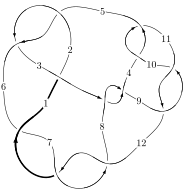
\includegraphics[width=112pt]{../../../GIT/diagram.site/Diagrams/png/1103_12a_0302.png}\\
\ \ \ A knot diagram\footnotemark}&
\allowdisplaybreaks
\textbf{Linearized knot diagam} \\
\cline{2-2}
 &
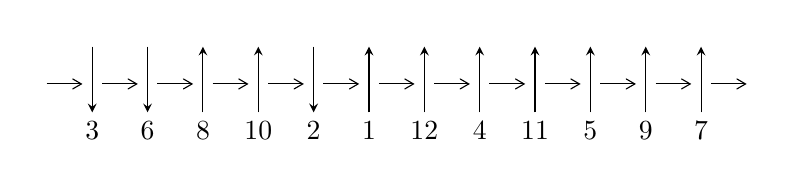
\begin{tikzpicture}[x=20pt, y=17pt]
	% nodes
	\node (C0) at (0, 0) {};
	\node (C1) at (1, 0) {};
	\node (C1U) at (1, +1) {};
	\node (C1D) at (1, -1) {3};

	\node (C2) at (2, 0) {};
	\node (C2U) at (2, +1) {};
	\node (C2D) at (2, -1) {6};

	\node (C3) at (3, 0) {};
	\node (C3U) at (3, +1) {};
	\node (C3D) at (3, -1) {8};

	\node (C4) at (4, 0) {};
	\node (C4U) at (4, +1) {};
	\node (C4D) at (4, -1) {10};

	\node (C5) at (5, 0) {};
	\node (C5U) at (5, +1) {};
	\node (C5D) at (5, -1) {2};

	\node (C6) at (6, 0) {};
	\node (C6U) at (6, +1) {};
	\node (C6D) at (6, -1) {1};

	\node (C7) at (7, 0) {};
	\node (C7U) at (7, +1) {};
	\node (C7D) at (7, -1) {12};

	\node (C8) at (8, 0) {};
	\node (C8U) at (8, +1) {};
	\node (C8D) at (8, -1) {4};

	\node (C9) at (9, 0) {};
	\node (C9U) at (9, +1) {};
	\node (C9D) at (9, -1) {11};

	\node (C10) at (10, 0) {};
	\node (C10U) at (10, +1) {};
	\node (C10D) at (10, -1) {5};

	\node (C11) at (11, 0) {};
	\node (C11U) at (11, +1) {};
	\node (C11D) at (11, -1) {9};

	\node (C12) at (12, 0) {};
	\node (C12U) at (12, +1) {};
	\node (C12D) at (12, -1) {7};
	\node (C13) at (13, 0) {};

	% arrows
	\draw[->,>={angle 60}]
	(C0) edge (C1) (C1) edge (C2) (C2) edge (C3) (C3) edge (C4) (C4) edge (C5) (C5) edge (C6) (C6) edge (C7) (C7) edge (C8) (C8) edge (C9) (C9) edge (C10) (C10) edge (C11) (C11) edge (C12) (C12) edge (C13) ;	\draw[->,>=stealth]
	(C1U) edge (C1D) (C2U) edge (C2D) (C3D) edge (C3U) (C4D) edge (C4U) (C5U) edge (C5D) (C6D) edge (C6U) (C7D) edge (C7U) (C8D) edge (C8U) (C9D) edge (C9U) (C10D) edge (C10U) (C11D) edge (C11U) (C12D) edge (C12U) ;
	\end{tikzpicture} \\
\hhline{~~} \\& 
\textbf{Solving Sequence} \\ \cline{2-2} 
 &
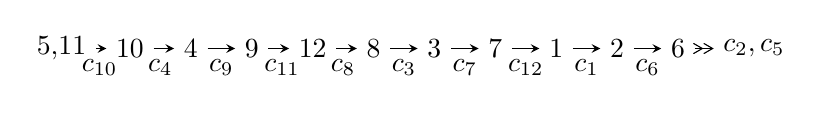
\begin{tikzpicture}[x=22pt, y=7pt]
	% node
	\node (A0) at (-1/8, 0) {5,11};
	\node (A1) at (1, 0) {10};
	\node (A2) at (2, 0) {4};
	\node (A3) at (3, 0) {9};
	\node (A4) at (4, 0) {12};
	\node (A5) at (5, 0) {8};
	\node (A6) at (6, 0) {3};
	\node (A7) at (7, 0) {7};
	\node (A8) at (8, 0) {1};
	\node (A9) at (9, 0) {2};
	\node (A10) at (10, 0) {6};
	\node (C1) at (1/2, -1) {$c_{10}$};
	\node (C2) at (3/2, -1) {$c_{4}$};
	\node (C3) at (5/2, -1) {$c_{9}$};
	\node (C4) at (7/2, -1) {$c_{11}$};
	\node (C5) at (9/2, -1) {$c_{8}$};
	\node (C6) at (11/2, -1) {$c_{3}$};
	\node (C7) at (13/2, -1) {$c_{7}$};
	\node (C8) at (15/2, -1) {$c_{12}$};
	\node (C9) at (17/2, -1) {$c_{1}$};
	\node (C10) at (19/2, -1) {$c_{6}$};
	\node (A11) at (45/4, 0) {$c_{2},c_{5}$};

	% edge
	\draw[->,>=stealth]	
	(A0) edge (A1) (A1) edge (A2) (A2) edge (A3) (A3) edge (A4) (A4) edge (A5) (A5) edge (A6) (A6) edge (A7) (A7) edge (A8) (A8) edge (A9) (A9) edge (A10) ;
	\draw[->>,>={angle 60}]	
	(A10) edge (A11);
\end{tikzpicture} \\ 

\end{tabular} \\

\footnotetext{
The image of knot diagram is generated by the software ``\textbf{Draw programme}" developed by Andrew Bartholomew(\url{http://www.layer8.co.uk/maths/draw/index.htm\#Running-draw}), where we modified some parts for our purpose(\url{https://github.com/CATsTAILs/LinksPainter}).
}\phantom \\ \newline 
\centering \textbf{Ideals for irreducible components\footnotemark of $X_{\text{par}}$} 
 
\begin{align*}
I^u_{1}&=\langle 
u^{72}-12 u^{70}+\cdots-2 u^2+1\rangle \\
I^u_{2}&=\langle 
u-1\rangle \\
\\
\end{align*}
\raggedright * 2 irreducible components of $\dim_{\mathbb{C}}=0$, with total 73 representations.\\
\footnotetext{All coefficients of polynomials are rational numbers. But the coefficients are sometimes approximated in decimal forms when there is not enough margin.}
\newpage
\renewcommand{\arraystretch}{1}
\centering \section*{I. $I^u_{1}= \langle u^{72}-12 u^{70}+\cdots-2 u^2+1 \rangle$}
\flushleft \textbf{(i) Arc colorings}\\
\begin{tabular}{m{7pt} m{180pt} m{7pt} m{180pt} }
\flushright $a_{5}=$&$\begin{pmatrix}0\\u\end{pmatrix}$ \\
\flushright $a_{11}=$&$\begin{pmatrix}1\\0\end{pmatrix}$ \\
\flushright $a_{10}=$&$\begin{pmatrix}1\\u^2\end{pmatrix}$ \\
\flushright $a_{4}=$&$\begin{pmatrix}- u\\- u^3+u\end{pmatrix}$ \\
\flushright $a_{9}=$&$\begin{pmatrix}- u^2+1\\u^2\end{pmatrix}$ \\
\flushright $a_{12}=$&$\begin{pmatrix}u^4- u^2+1\\- u^4\end{pmatrix}$ \\
\flushright $a_{8}=$&$\begin{pmatrix}- u^6+u^4-2 u^2+1\\- u^8+2 u^6-2 u^4+2 u^2\end{pmatrix}$ \\
\flushright $a_{3}=$&$\begin{pmatrix}u^{11}-2 u^9+4 u^7-4 u^5+3 u^3-2 u\\u^{13}-3 u^{11}+5 u^9-6 u^7+4 u^5-3 u^3+u\end{pmatrix}$ \\
\flushright $a_{7}=$&$\begin{pmatrix}u^{16}-3 u^{14}+7 u^{12}-10 u^{10}+11 u^8-10 u^6+6 u^4-4 u^2+1\\- u^{16}+2 u^{14}-4 u^{12}+4 u^{10}-4 u^8+4 u^6-2 u^4+2 u^2\end{pmatrix}$ \\
\flushright $a_{1}=$&$\begin{pmatrix}u^{28}-5 u^{26}+\cdots-3 u^2+1\\- u^{28}+4 u^{26}+\cdots+10 u^6-5 u^4\end{pmatrix}$ \\
\flushright $a_{2}=$&$\begin{pmatrix}u^{52}-9 u^{50}+\cdots-5 u^2+1\\u^{54}-10 u^{52}+\cdots-14 u^4+u^2\end{pmatrix}$ \\
\flushright $a_{6}=$&$\begin{pmatrix}u^{40}-7 u^{38}+\cdots-6 u^2+1\\- u^{40}+6 u^{38}+\cdots-2 u^4+2 u^2\end{pmatrix}$\\&\end{tabular}
\flushleft \textbf{(ii) Obstruction class $= -1$}\\~\\
\flushleft \textbf{(iii) Cusp Shapes $= -4 u^{70}+44 u^{68}+\cdots+12 u+6$}\\~\\
\newpage\renewcommand{\arraystretch}{1}
\flushleft \textbf{(iv) u-Polynomials at the component}\newline \\
\begin{tabular}{m{50pt}|m{274pt}}
Crossings & \hspace{64pt}u-Polynomials at each crossing \\
\hline $$\begin{aligned}c_{1}\end{aligned}$$&$\begin{aligned}
&u^{72}+40 u^{71}+\cdots+4 u+1
\end{aligned}$\\
\hline $$\begin{aligned}c_{2},c_{5}\end{aligned}$$&$\begin{aligned}
&u^{72}+2 u^{71}+\cdots-2 u^2+1
\end{aligned}$\\
\hline $$\begin{aligned}c_{3},c_{8}\end{aligned}$$&$\begin{aligned}
&u^{72}+2 u^{71}+\cdots+170 u+25
\end{aligned}$\\
\hline $$\begin{aligned}c_{4},c_{10}\end{aligned}$$&$\begin{aligned}
&u^{72}-12 u^{70}+\cdots-2 u^2+1
\end{aligned}$\\
\hline $$\begin{aligned}c_{6},c_{7},c_{12}\end{aligned}$$&$\begin{aligned}
&u^{72}+3 u^{71}+\cdots+32 u+17
\end{aligned}$\\
\hline $$\begin{aligned}c_{9},c_{11}\end{aligned}$$&$\begin{aligned}
&u^{72}-24 u^{71}+\cdots-4 u+1
\end{aligned}$\\
\hline
\end{tabular}\\~\\
\newpage\renewcommand{\arraystretch}{1}
\flushleft \textbf{(v) Riley Polynomials at the component}\newline \\
\begin{tabular}{m{50pt}|m{274pt}}
Crossings & \hspace{64pt}Riley Polynomials at each crossing \\
\hline $$\begin{aligned}c_{1}\end{aligned}$$&$\begin{aligned}
&y^{72}-16 y^{71}+\cdots-4 y+1
\end{aligned}$\\
\hline $$\begin{aligned}c_{2},c_{5}\end{aligned}$$&$\begin{aligned}
&y^{72}-40 y^{71}+\cdots-4 y+1
\end{aligned}$\\
\hline $$\begin{aligned}c_{3},c_{8}\end{aligned}$$&$\begin{aligned}
&y^{72}-36 y^{71}+\cdots-28800 y+625
\end{aligned}$\\
\hline $$\begin{aligned}c_{4},c_{10}\end{aligned}$$&$\begin{aligned}
&y^{72}-24 y^{71}+\cdots-4 y+1
\end{aligned}$\\
\hline $$\begin{aligned}c_{6},c_{7},c_{12}\end{aligned}$$&$\begin{aligned}
&y^{72}+75 y^{71}+\cdots+16180 y+289
\end{aligned}$\\
\hline $$\begin{aligned}c_{9},c_{11}\end{aligned}$$&$\begin{aligned}
&y^{72}+48 y^{71}+\cdots+12 y+1
\end{aligned}$\\
\hline
\end{tabular}\\~\\
\newpage\flushleft \textbf{(vi) Complex Volumes and Cusp Shapes}
$$\begin{array}{c|c|c}  
\text{Solutions to }I^u_{1}& \I (\text{vol} + \sqrt{-1}CS) & \text{Cusp shape}\\
 \hline 
\begin{aligned}
u &= -0.685263 + 0.729392 I\end{aligned}
 & -3.50695 + 0.02726 I & -1.83210 + 0. I\phantom{ +0.000000I} \\ \hline\begin{aligned}
u &= -0.685263 - 0.729392 I\end{aligned}
 & -3.50695 - 0.02726 I & -1.83210 + 0. I\phantom{ +0.000000I} \\ \hline\begin{aligned}
u &= -0.616766 + 0.759182 I\end{aligned}
 & -0.97423 + 5.55134 I & \phantom{-}3.79833 - 6.21492 I \\ \hline\begin{aligned}
u &= -0.616766 - 0.759182 I\end{aligned}
 & -0.97423 - 5.55134 I & \phantom{-}3.79833 + 6.21492 I \\ \hline\begin{aligned}
u &= -0.646232 + 0.799441 I\end{aligned}
 & -5.48260 + 4.68989 I & \phantom{-}6.00000 + 0. I\phantom{ +0.000000I} \\ \hline\begin{aligned}
u &= -0.646232 - 0.799441 I\end{aligned}
 & -5.48260 - 4.68989 I & \phantom{-}6.00000 + 0. I\phantom{ +0.000000I} \\ \hline\begin{aligned}
u &= \phantom{-}0.642592 + 0.806323 I\end{aligned}
 & -8.95862 - 9.56030 I & \phantom{-0.000000 } 0 \\ \hline\begin{aligned}
u &= \phantom{-}0.642592 - 0.806323 I\end{aligned}
 & -8.95862 + 9.56030 I & \phantom{-0.000000 } 0 \\ \hline\begin{aligned}
u &= \phantom{-}0.655486 + 0.801847 I\end{aligned}
 & -9.46744 - 0.22227 I & \phantom{-0.000000 } 0 \\ \hline\begin{aligned}
u &= \phantom{-}0.655486 - 0.801847 I\end{aligned}
 & -9.46744 + 0.22227 I & \phantom{-0.000000 } 0 \\ \hline\begin{aligned}
u &= \phantom{-}0.614794 + 0.726778 I\end{aligned}
 & \phantom{-}0.52664 - 1.37080 I & \phantom{-}7.44043 + 0.82909 I \\ \hline\begin{aligned}
u &= \phantom{-}0.614794 - 0.726778 I\end{aligned}
 & \phantom{-}0.52664 + 1.37080 I & \phantom{-}7.44043 - 0.82909 I \\ \hline\begin{aligned}
u &= -0.842454 + 0.642342 I\end{aligned}
 & -2.01813 - 2.49648 I & \phantom{-0.000000 } 0 \\ \hline\begin{aligned}
u &= -0.842454 - 0.642342 I\end{aligned}
 & -2.01813 + 2.49648 I & \phantom{-0.000000 } 0 \\ \hline\begin{aligned}
u &= -1.070910 + 0.017521 I\end{aligned}
 & \phantom{-}5.97297 - 0.60288 I & \phantom{-0.000000 } 0 \\ \hline\begin{aligned}
u &= -1.070910 - 0.017521 I\end{aligned}
 & \phantom{-}5.97297 + 0.60288 I & \phantom{-0.000000 } 0 \\ \hline\begin{aligned}
u &= -1.067600 + 0.102765 I\end{aligned}
 & -3.24294 + 0.10414 I & \phantom{-0.000000 } 0 \\ \hline\begin{aligned}
u &= -1.067600 - 0.102765 I\end{aligned}
 & -3.24294 - 0.10414 I & \phantom{-0.000000 } 0 \\ \hline\begin{aligned}
u &= \phantom{-}0.808140 + 0.711304 I\end{aligned}
 & -5.02712 - 0.48220 I & \phantom{-0.000000 } 0 \\ \hline\begin{aligned}
u &= \phantom{-}0.808140 - 0.711304 I\end{aligned}
 & -5.02712 + 0.48220 I & \phantom{-0.000000 } 0 \\ \hline\begin{aligned}
u &= \phantom{-}1.077510 + 0.040400 I\end{aligned}
 & \phantom{-}4.74846 + 4.83042 I & \phantom{-0.000000 } 0 \\ \hline\begin{aligned}
u &= \phantom{-}1.077510 - 0.040400 I\end{aligned}
 & \phantom{-}4.74846 - 4.83042 I & \phantom{-0.000000 } 0 \\ \hline\begin{aligned}
u &= \phantom{-}1.074930 + 0.090664 I\end{aligned}
 & \phantom{-}0.68708 + 4.24895 I & \phantom{-0.000000 } 0 \\ \hline\begin{aligned}
u &= \phantom{-}1.074930 - 0.090664 I\end{aligned}
 & \phantom{-}0.68708 - 4.24895 I & \phantom{-0.000000 } 0 \\ \hline\begin{aligned}
u &= -1.084780 + 0.094266 I\end{aligned}
 & -2.71190 - 9.05881 I & \phantom{-0.000000 } 0 \\ \hline\begin{aligned}
u &= -1.084780 - 0.094266 I\end{aligned}
 & -2.71190 + 9.05881 I & \phantom{-0.000000 } 0 \\ \hline\begin{aligned}
u &= \phantom{-}0.964081 + 0.532824 I\end{aligned}
 & -5.75145 + 6.22706 I & \phantom{-0.000000 } 0 \\ \hline\begin{aligned}
u &= \phantom{-}0.964081 - 0.532824 I\end{aligned}
 & -5.75145 - 6.22706 I & \phantom{-0.000000 } 0 \\ \hline\begin{aligned}
u &= \phantom{-}0.588986 + 0.660789 I\end{aligned}
 & \phantom{-}0.924456 - 0.405677 I & \phantom{-}8.51154 + 0.82456 I \\ \hline\begin{aligned}
u &= \phantom{-}0.588986 - 0.660789 I\end{aligned}
 & \phantom{-}0.924456 + 0.405677 I & \phantom{-}8.51154 - 0.82456 I\\
 \hline 
 \end{array}$$\newpage$$\begin{array}{c|c|c}  
\text{Solutions to }I^u_{1}& \I (\text{vol} + \sqrt{-1}CS) & \text{Cusp shape}\\
 \hline 
\begin{aligned}
u &= -0.971960 + 0.563675 I\end{aligned}
 & -2.07865 - 1.92425 I & \phantom{-0.000000 } 0 \\ \hline\begin{aligned}
u &= -0.971960 - 0.563675 I\end{aligned}
 & -2.07865 + 1.92425 I & \phantom{-0.000000 } 0 \\ \hline\begin{aligned}
u &= \phantom{-}0.895218 + 0.693491 I\end{aligned}
 & -4.75836 + 5.86106 I & \phantom{-0.000000 } 0 \\ \hline\begin{aligned}
u &= \phantom{-}0.895218 - 0.693491 I\end{aligned}
 & -4.75836 - 5.86106 I & \phantom{-0.000000 } 0 \\ \hline\begin{aligned}
u &= \phantom{-}0.992256 + 0.556250 I\end{aligned}
 & -5.45230 - 2.69823 I & \phantom{-0.000000 } 0 \\ \hline\begin{aligned}
u &= \phantom{-}0.992256 - 0.556250 I\end{aligned}
 & -5.45230 + 2.69823 I & \phantom{-0.000000 } 0 \\ \hline\begin{aligned}
u &= \phantom{-}0.867105 + 0.759891 I\end{aligned}
 & -9.07437 + 2.86581 I & \phantom{-0.000000 } 0 \\ \hline\begin{aligned}
u &= \phantom{-}0.867105 - 0.759891 I\end{aligned}
 & -9.07437 - 2.86581 I & \phantom{-0.000000 } 0 \\ \hline\begin{aligned}
u &= -0.862009 + 0.766282 I\end{aligned}
 & -12.84810 + 1.84355 I & \phantom{-0.000000 } 0 \\ \hline\begin{aligned}
u &= -0.862009 - 0.766282 I\end{aligned}
 & -12.84810 - 1.84355 I & \phantom{-0.000000 } 0 \\ \hline\begin{aligned}
u &= -0.874376 + 0.763198 I\end{aligned}
 & -12.8104 - 7.6046 I & \phantom{-0.000000 } 0 \\ \hline\begin{aligned}
u &= -0.874376 - 0.763198 I\end{aligned}
 & -12.8104 + 7.6046 I & \phantom{-0.000000 } 0 \\ \hline\begin{aligned}
u &= -0.730912 + 0.402422 I\end{aligned}
 & -0.11472 - 3.40202 I & \phantom{-}7.20877 + 8.25970 I \\ \hline\begin{aligned}
u &= -0.730912 - 0.402422 I\end{aligned}
 & -0.11472 + 3.40202 I & \phantom{-}7.20877 - 8.25970 I \\ \hline\begin{aligned}
u &= -1.004080 + 0.624647 I\end{aligned}
 & \phantom{-}1.20214 - 1.36853 I & \phantom{-0.000000 } 0 \\ \hline\begin{aligned}
u &= -1.004080 - 0.624647 I\end{aligned}
 & \phantom{-}1.20214 + 1.36853 I & \phantom{-0.000000 } 0 \\ \hline\begin{aligned}
u &= \phantom{-}1.009180 + 0.644267 I\end{aligned}
 & \phantom{-}2.12034 + 5.52640 I & \phantom{-0.000000 } 0 \\ \hline\begin{aligned}
u &= \phantom{-}1.009180 - 0.644267 I\end{aligned}
 & \phantom{-}2.12034 - 5.52640 I & \phantom{-0.000000 } 0 \\ \hline\begin{aligned}
u &= -0.990350 + 0.679412 I\end{aligned}
 & -2.58830 - 5.42724 I & \phantom{-0.000000 } 0 \\ \hline\begin{aligned}
u &= -0.990350 - 0.679412 I\end{aligned}
 & -2.58830 + 5.42724 I & \phantom{-0.000000 } 0 \\ \hline\begin{aligned}
u &= \phantom{-}1.016670 + 0.666187 I\end{aligned}
 & \phantom{-}1.70598 + 6.71869 I & \phantom{-0.000000 } 0 \\ \hline\begin{aligned}
u &= \phantom{-}1.016670 - 0.666187 I\end{aligned}
 & \phantom{-}1.70598 - 6.71869 I & \phantom{-0.000000 } 0 \\ \hline\begin{aligned}
u &= -1.024170 + 0.676591 I\end{aligned}
 & \phantom{-}0.23261 - 11.01360 I & \phantom{-0.000000 } 0 \\ \hline\begin{aligned}
u &= -1.024170 - 0.676591 I\end{aligned}
 & \phantom{-}0.23261 + 11.01360 I & \phantom{-0.000000 } 0 \\ \hline\begin{aligned}
u &= -0.501415 + 0.583380 I\end{aligned}
 & -0.06144 - 3.50578 I & \phantom{-}5.32142 + 7.03074 I \\ \hline\begin{aligned}
u &= -0.501415 - 0.583380 I\end{aligned}
 & -0.06144 + 3.50578 I & \phantom{-}5.32142 - 7.03074 I \\ \hline\begin{aligned}
u &= \phantom{-}1.022920 + 0.704607 I\end{aligned}
 & -8.35859 + 5.89706 I & \phantom{-0.000000 } 0 \\ \hline\begin{aligned}
u &= \phantom{-}1.022920 - 0.704607 I\end{aligned}
 & -8.35859 - 5.89706 I & \phantom{-0.000000 } 0 \\ \hline\begin{aligned}
u &= -1.026150 + 0.700458 I\end{aligned}
 & -4.33826 - 10.34330 I & \phantom{-0.000000 } 0 \\ \hline\begin{aligned}
u &= -1.026150 - 0.700458 I\end{aligned}
 & -4.33826 + 10.34330 I & \phantom{-0.000000 } 0\\
 \hline 
 \end{array}$$\newpage$$\begin{array}{c|c|c}  
\text{Solutions to }I^u_{1}& \I (\text{vol} + \sqrt{-1}CS) & \text{Cusp shape}\\
 \hline 
\begin{aligned}
u &= \phantom{-}1.029980 + 0.702080 I\end{aligned}
 & -7.7907 + 15.2371 I & \phantom{-0.000000 } 0 \\ \hline\begin{aligned}
u &= \phantom{-}1.029980 - 0.702080 I\end{aligned}
 & -7.7907 - 15.2371 I & \phantom{-0.000000 } 0 \\ \hline\begin{aligned}
u &= \phantom{-}0.308780 + 0.639750 I\end{aligned}
 & -7.21219 + 7.05768 I & -0.07616 - 5.90453 I \\ \hline\begin{aligned}
u &= \phantom{-}0.308780 - 0.639750 I\end{aligned}
 & -7.21219 - 7.05768 I & -0.07616 + 5.90453 I \\ \hline\begin{aligned}
u &= -0.302317 + 0.614260 I\end{aligned}
 & -3.72314 - 2.33103 I & \phantom{-}2.90552 + 2.90095 I \\ \hline\begin{aligned}
u &= -0.302317 - 0.614260 I\end{aligned}
 & -3.72314 + 2.33103 I & \phantom{-}2.90552 - 2.90095 I \\ \hline\begin{aligned}
u &= \phantom{-}0.271854 + 0.619380 I\end{aligned}
 & -7.53422 - 2.12033 I & -0.914618 + 0.535660 I \\ \hline\begin{aligned}
u &= \phantom{-}0.271854 - 0.619380 I\end{aligned}
 & -7.53422 + 2.12033 I & -0.914618 - 0.535660 I \\ \hline\begin{aligned}
u &= \phantom{-}0.607470 + 0.101465 I\end{aligned}
 & \phantom{-}0.893845 + 0.072656 I & \phantom{-}11.83691 - 0.70837 I \\ \hline\begin{aligned}
u &= \phantom{-}0.607470 - 0.101465 I\end{aligned}
 & \phantom{-}0.893845 - 0.072656 I & \phantom{-}11.83691 + 0.70837 I \\ \hline\begin{aligned}
u &= -0.146204 + 0.400346 I\end{aligned}
 & -1.56463 + 0.90785 I & -1.88769 - 0.68738 I \\ \hline\begin{aligned}
u &= -0.146204 - 0.400346 I\end{aligned}
 & -1.56463 - 0.90785 I & -1.88769 + 0.68738 I\\
 \hline 
 \end{array}$$\newpage\newpage\renewcommand{\arraystretch}{1}
\centering \section*{II. $I^u_{2}= \langle u-1 \rangle$}
\flushleft \textbf{(i) Arc colorings}\\
\begin{tabular}{m{7pt} m{180pt} m{7pt} m{180pt} }
\flushright $a_{5}=$&$\begin{pmatrix}0\\1\end{pmatrix}$ \\
\flushright $a_{11}=$&$\begin{pmatrix}1\\0\end{pmatrix}$ \\
\flushright $a_{10}=$&$\begin{pmatrix}1\\1\end{pmatrix}$ \\
\flushright $a_{4}=$&$\begin{pmatrix}-1\\0\end{pmatrix}$ \\
\flushright $a_{9}=$&$\begin{pmatrix}0\\1\end{pmatrix}$ \\
\flushright $a_{12}=$&$\begin{pmatrix}1\\-1\end{pmatrix}$ \\
\flushright $a_{8}=$&$\begin{pmatrix}-1\\1\end{pmatrix}$ \\
\flushright $a_{3}=$&$\begin{pmatrix}0\\-1\end{pmatrix}$ \\
\flushright $a_{7}=$&$\begin{pmatrix}-1\\1\end{pmatrix}$ \\
\flushright $a_{1}=$&$\begin{pmatrix}1\\-1\end{pmatrix}$ \\
\flushright $a_{2}=$&$\begin{pmatrix}1\\0\end{pmatrix}$ \\
\flushright $a_{6}=$&$\begin{pmatrix}-1\\1\end{pmatrix}$\\&\end{tabular}
\flushleft \textbf{(ii) Obstruction class $= -1$}\\~\\
\flushleft \textbf{(iii) Cusp Shapes $= 6$}\\~\\
\newpage\renewcommand{\arraystretch}{1}
\flushleft \textbf{(iv) u-Polynomials at the component}\newline \\
\begin{tabular}{m{50pt}|m{274pt}}
Crossings & \hspace{64pt}u-Polynomials at each crossing \\
\hline $$\begin{aligned}c_{1}\end{aligned}$$&$\begin{aligned}
&u+1
\end{aligned}$\\
\hline $$\begin{aligned}c_{2},c_{3},c_{4}\\c_{5},c_{8},c_{9}\\c_{10},c_{11}\end{aligned}$$&$\begin{aligned}
&u-1
\end{aligned}$\\
\hline $$\begin{aligned}c_{6},c_{7},c_{12}\end{aligned}$$&$\begin{aligned}
&u
\end{aligned}$\\
\hline
\end{tabular}\\~\\
\newpage\renewcommand{\arraystretch}{1}
\flushleft \textbf{(v) Riley Polynomials at the component}\newline \\
\begin{tabular}{m{50pt}|m{274pt}}
Crossings & \hspace{64pt}Riley Polynomials at each crossing \\
\hline $$\begin{aligned}c_{1},c_{2},c_{3}\\c_{4},c_{5},c_{8}\\c_{9},c_{10},c_{11}\end{aligned}$$&$\begin{aligned}
&y-1
\end{aligned}$\\
\hline $$\begin{aligned}c_{6},c_{7},c_{12}\end{aligned}$$&$\begin{aligned}
&y
\end{aligned}$\\
\hline
\end{tabular}\\~\\
\newpage\flushleft \textbf{(vi) Complex Volumes and Cusp Shapes}
$$\begin{array}{c|c|c}  
\text{Solutions to }I^u_{2}& \I (\text{vol} + \sqrt{-1}CS) & \text{Cusp shape}\\
 \hline 
\begin{aligned}
u &= \phantom{-}1.00000\phantom{ +0.000000I}\end{aligned}
 & \phantom{-}1.64493\phantom{ +0.000000I} & \phantom{-}6.00000\phantom{ +0.000000I}\\
 \hline 
 \end{array}$$\newpage
\newpage\renewcommand{\arraystretch}{1}
\centering \section*{ III. u-Polynomials}
\begin{tabular}{m{50pt}|m{274pt}}
Crossings & \hspace{64pt}u-Polynomials at each crossing \\
\hline $$\begin{aligned}c_{1}\end{aligned}$$&$\begin{aligned}
&(u+1)(u^{72}+40 u^{71}+\cdots+4 u+1)
\end{aligned}$\\
\hline $$\begin{aligned}c_{2},c_{5}\end{aligned}$$&$\begin{aligned}
&(u-1)(u^{72}+2 u^{71}+\cdots-2 u^2+1)
\end{aligned}$\\
\hline $$\begin{aligned}c_{3},c_{8}\end{aligned}$$&$\begin{aligned}
&(u-1)(u^{72}+2 u^{71}+\cdots+170 u+25)
\end{aligned}$\\
\hline $$\begin{aligned}c_{4},c_{10}\end{aligned}$$&$\begin{aligned}
&(u-1)(u^{72}-12 u^{70}+\cdots-2 u^2+1)
\end{aligned}$\\
\hline $$\begin{aligned}c_{6},c_{7},c_{12}\end{aligned}$$&$\begin{aligned}
&u(u^{72}+3 u^{71}+\cdots+32 u+17)
\end{aligned}$\\
\hline $$\begin{aligned}c_{9},c_{11}\end{aligned}$$&$\begin{aligned}
&(u-1)(u^{72}-24 u^{71}+\cdots-4 u+1)
\end{aligned}$\\
\hline
\end{tabular}\newpage\renewcommand{\arraystretch}{1}
\centering \section*{ IV. Riley Polynomials}
\begin{tabular}{m{50pt}|m{274pt}}
Crossings & \hspace{64pt}Riley Polynomials at each crossing \\
\hline $$\begin{aligned}c_{1}\end{aligned}$$&$\begin{aligned}
&(y-1)(y^{72}-16 y^{71}+\cdots-4 y+1)
\end{aligned}$\\
\hline $$\begin{aligned}c_{2},c_{5}\end{aligned}$$&$\begin{aligned}
&(y-1)(y^{72}-40 y^{71}+\cdots-4 y+1)
\end{aligned}$\\
\hline $$\begin{aligned}c_{3},c_{8}\end{aligned}$$&$\begin{aligned}
&(y-1)(y^{72}-36 y^{71}+\cdots-28800 y+625)
\end{aligned}$\\
\hline $$\begin{aligned}c_{4},c_{10}\end{aligned}$$&$\begin{aligned}
&(y-1)(y^{72}-24 y^{71}+\cdots-4 y+1)
\end{aligned}$\\
\hline $$\begin{aligned}c_{6},c_{7},c_{12}\end{aligned}$$&$\begin{aligned}
&y(y^{72}+75 y^{71}+\cdots+16180 y+289)
\end{aligned}$\\
\hline $$\begin{aligned}c_{9},c_{11}\end{aligned}$$&$\begin{aligned}
&(y-1)(y^{72}+48 y^{71}+\cdots+12 y+1)
\end{aligned}$\\
\hline
\end{tabular}
\vskip 2pc
\end{document}